%\documentclass[12pt,a4paper]{article}
\usepackage{xeCJK}
\usepackage{fancyhdr}%页眉页脚
\usepackage{listings}%代码块
\usepackage[margin=1in]{geometry}%页边距
\usepackage{graphics}%图片
\usepackage{fontspec}
\usepackage{amsmath}
\usepackage{amsfonts}
\usepackage{eqnarray}
\usepackage{tabularx}
%定义页眉页脚
\pagestyle{fancy}
\fancyhf{}
\fancyhead[C]{\selectfont \textsc{ACM Template}}
\fancyhead[L]{\rightmark}
\fancyhead[R]{Geometry Rhythm}
%\lfoot{lfoot}
%\cfoot{qkoqhh}
\rfoot{\thepage}
%\renewcommand{\footrulewidth}{0.5pt}

%\rmfamily%罗马字体




\lstset{
	language=C,%代码的语言
	numbers=left,%行号
	frame=single,%
	basicstyle=\footnotesize,
	extendedchars=false,
	basicstyle=\small\ttfamily,
	%	tabsize=2,
	breaklines=true,
	showstringspaces=false
}



\title{ACM Template}
\author{qkoqhh}
%\begin{document}
	\newpage
	\section{图论}
	\subsection{最短路}
	\subsubsection*{dijkstra}
	\lstinputlisting{./source/dijkstra.cpp}
	\vspace{2cm}
	\subsubsection*{SPFA}
	\lstinputlisting{./source/spfa.cpp}
	\newpage
	\subsection{tarjan缩环}
	{\large 这里仅给出有向图缩环}\\
	\lstinputlisting{./source/tarjan.cpp}
	\newpage
	\subsection{有向基环树}
	{\large 利用tarjan找出基环}\\
	\lstinputlisting{./source/tree1.cpp}
	\newpage
	\subsection{无向基环树}
	{\large 细节情况巨多,容易写挫}\\
	\lstinputlisting{./source/tree2.cpp}
	\newpage
	\subsection{点分治}
	{\large 一个简单的例子,主要是写点分的姿势和一些固定的功能函数}\\
	\lstinputlisting{./source/div.cpp}
	\newpage
	\subsection{fleury算法}
	主要用于求解欧拉路径及其输出方案\vspace{0.3cm}\\
	{\small 例题:求无向图最小路径覆盖\\	
	与有向图的二分图做法不同,这个要转化为求最少的欧拉路径\\
	有个结论是欧拉路径的个数为度为奇数的点的个数/2(类比欧拉回路的结论)\\	
	然后求欧拉路径的方法是fleury算法。。其思想就是暴力dfs,然后巧妙的地方就是边是反向取的,即以出栈的顺序为欧拉路径。。\\
	然后就是一大堆细节问题,需要全面考虑(偶数的欧拉回路,奇数的欧拉回路和欧拉路径、分块求欧拉路径等)\\}
	\lstinputlisting{./source/fleury.cpp}
	\newpage
	\subsection{k短路}
	{\large A*算法}\\
	\lstinputlisting{./source/k-short.cpp}
	\newpage
	\subsection{对偶图}
	\subsubsection{定义}~

	 一个图 $G=(V,E)$,若能将其画在平面上,且任意两条边的交点只能是 $G$ 的顶点,则称 $G$ 可嵌入平面,或称 $G$ 是可平面的。可平面图在平面上的一个嵌入称为一个平面图。如下图左边两图为平面图,右边两图不属于平面图:\\
	 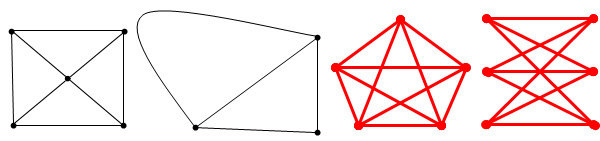
\includegraphics[scale=0.75]{./source/img1.jpeg}
	 
	 由平面图的边包围而成,其中不含图的顶点。也称为面。包围面 $R$ 的所有边组成的回路称为该面的边界,回路长度称为该面的度,记为 $deg(R)$。具有相同边界的面称为相邻面。由平面图的边包围且无穷大的面称为外部面。一个平面图有且只有一个外部面。如下面的平面图中,$R_0$ 是外部面 $R_0$ 与 $R_1,R_2,R_3$ 均相邻。$deg(R_0)=8$, $deg(R_1)=4$,$deg(R_2)=5$($R_2$ 经过的顶点序列为 $v_7\rightarrow v_4\rightarrow v_6\rightarrow v_4\rightarrow v_5\rightarrow v_7$ ), $deg(R_3)=1$:\\
	 \begin{center}
	 	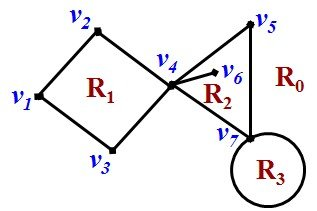
\includegraphics[scale=0.5]{./source/img2.jpeg}
	 \end{center}
	 
	利用欧拉公式和数学归纳法可以证明平面图G的所有面的度之和等于其边数 $\left|E\right|$ 的 $2$ 倍,即:
	$$
	\sum_{i=1}^{r}deg(R_i)=2\left|E|\right|
	$$
	
	下面我们引入对偶图,设有平面图 $G=(V,E)$,满足下列条件的图$G'=(V',E')$ 称为图 $G$ 的对偶图:$G$ 的任一面 $R_i$ 内有且仅有一点 $V_i'$;对 $G$ 的域 $R_i$ 和 $R_j$ 的共同边界 $E_k$,画一条边 $E_k'=(V_i',V_j')$ 且只与 $E_k$ 交于一点;若 $E_k$ 完全处于 $R_i$ 中,则 $V_i'$ 有一自环 $E_k'$,如下图 $G'$ 是 $G$ 的对偶图:
	\begin{center}
		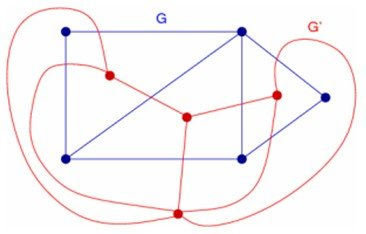
\includegraphics[scale=0.5]{./source/img3.jpeg}
	\end{center}
	\subsubsection{最大流的应用}~
	
	如果网络流中的图 $G$ 可以转化为一个平面图,那么其对偶图 $G'$ 中的环对应 $G$ 中的割,利用最大流最小割定理转化模型,根据平面图 $G'$ 与其对偶图的关系,先求出最小割。首先连接 $s$ 和 $t$,如下图蓝色虚线,得到一个附加面,我们设附加面对应的点为 $s'$,无界面对应的点为 $t'$,求该图的红色的对偶图 $G'$,最后删去 $s'$ 和 $t'$ 之间的边:
	\begin{center}
		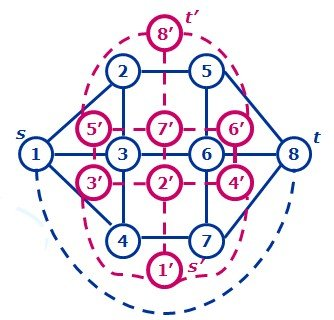
\includegraphics[scale=0.5]{./source/img4.jpeg}
	\end{center}
	
	一条从 $s'$ 到 $t'$ 的路径,就对应了一个 $s-t$ 割,更进一步,如果我们令每条边的长度等于它的容量,那么最小割的容量就等于最短路的长度。这样时间复杂度大大降低了对偶图的应用。\\
	\\
	\subsubsection{平面图和对偶图的关系}
	\begin{enumerate}
		\item $G^*$ 中的环与 $G$ 中的割一一对应.(割就是一些边, 如果割掉这些边使图分成两个互不连通的子图的话, 就称之为割).
		\item $G$ 的面数等于 $G^*$ 的点数,$G$ 与 $G^*$ 的边数相同.
	\end{enumerate}
	\newpage
	\subsection{三元环计数}~
	
	三元环计数的方法是将无向图变成有向图,对每条边,从度小的点连向度大的点,如果度相同则按编号的大小连边,这样保证了这个图是个 $DAG$ ,此时三元环就被表示成类似于 $G=\{(A,B,C),(AB,AC,BC)\}$ 这样的玩意
	
	然后枚举点 $u$,标记 $u$ 的出点。枚举 $u$ 的出边,再枚举出点 $v$ 的出边,然后如果 $v$ 的出点被标记,那么就必定形成一个三元环
	
	这个算法的复杂度是 $O(m^{1.5})$ ,证明如下:
	
	首先这个图中每个点的出度都不大于 $\sqrt{m}$ 。假设存在大于 $\sqrt{m}$ 的点,那么其出边也必然大于 $\sqrt{m}$ ,这样边数就大于 $m$ 了,矛盾。
	
	那么这样暴力的复杂度就是 $O(m^{1.5})$\\
	\lstinputlisting{./source/circle3.cpp}
	\newpage
	\subsection{Prufer序列}
	\subsubsection{定义}
	$Prufer$ 数列是无根树的一种数列。在组合数学中,$Prufer$ 数列由有一个对于顶点标过号的树转化来的数列,点数为 $n$ 的树转化来的 $Prufer$ 数列长度为 $n-2$。\\
	\subsubsection{构造方法}
	\paragraph{无根树转化为prufer序列}
	\begin{enumerate}
		\item 找到编号最小的度数为 $1$ 的点
		\item 删除该节点并在序列中添加与该节点相连的节点的编号
		\item 重复 $1,2$ 操作,直到整棵树只剩下两个节点
	\end{enumerate}
	如下图的 $prufer$ 序列为 $3,5,1,3$
	\begin{center}
		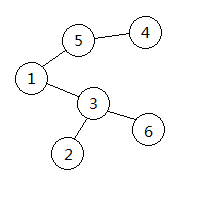
\includegraphics[scale=0.7]{./source/tree.png}
	\end{center}
	\paragraph{prufer序列转化为无根树}
	\begin{enumerate}
		\item 构造点集 $\{1,2,\cdots,n\}$
		\item 每次取出 $prufer$ 序列中最前面的元素 $u$
		\item 在点集中找到编号最小的没有在 $prufer$ 序列中出现的元素 $v$
		\item 给 $u,v$ 连边然后将 $u$ 从 $prufer$ 中删除,将 $v$ 从点集中删除
		\item 最后在点集中剩下两个节点,给它们连边
	\end{enumerate}
	例如,对于 $prufer$ 序列 $3,5,1,3$ 的连边顺序为 $(3,2),(5,4),(1,5),(3,1),(3,6)$\\
	\subsubsection{性质}
	\begin{enumerate}
		\item $prufer$ 序列中某个编号出现的次数就等于这个编号的节点在无根树中的度数 $-1$
		\item 一棵 $n$ 个节点的无根树唯一地对应了一个长度为 $n-2$ 的数列,数列中的每个数都在 $1$ 到 $n$ 的范围内。
		\item $n$ 个点的无向完全图的生成树的计数:$n(n-2)$,即 $n$ 个点的有标号无根树的计数
		\item $n$ 个节点的度依次为 $d_1,d_2,\cdots,d_n$ 的无根树共有 $\displaystyle \frac{(n-2)!}{\prod_{i=1}^{n}(d_i-1)}$ 个,因为此时Prufer编码中的数字 $i$ 恰好出现 $d_i-1$ 次,$(n-2)!$ 是总排列数
		\item $n$ 个点的有标号有根树的计数: $n^{(n-2)}*n = n^{(n-1)}$
	\end{enumerate}

	\newpage
	\subsection{其他建图技巧}
	\subsubsection{例题1}
	\paragraph{题意}~
	
	给出一个 $n$ 个点 $m$ 条边的无向图,经过一个点的代价是进入和离开这个点的两条边权的较大值,求从起点 $1$ 到点 $n$ 的最小代价。起点的代价是离开起点的边的边权,终点的代价是进入终点的边的边权。\\
	$n\le10^5,m\le10^5$
	\paragraph{题解}~
	
	可以把边看成点,然后有公共点的边相互连边,跑最短路就可以了。。
	
	然而菊花图会退化成 $m^2$ ,需要再优化。。
	
	把无向边拆成 $2$ 个有向边,对每个点存入边和出边,然后出边之间做个差分,即对出边的边权排序,然后相邻边之间连边,小边向大边连权值为2边权值之差的边,大边向小边连权值为0的边,这样入边只需向他的对应边连一个权值为原边权的边即可达到去最大值的效果。
	
	然后剩下起点和终点就直接想对应的出边和入边连边就行了,边权为原图的边权。。\\
	\subsubsection{例题2}
	\paragraph{题意}~
	
	给定平面上的 $n$ 个点,定义 $(x_1,y_1)$ 到 $(x_2,y_2)$ 的费用为 $\min\{|x_1-x_2|,|y_1-y_2|\}$,求从 $1$ 号点走到 $n$ 号点的最小费用。\\
	$n\le2\times10^5$
	\paragraph{题解}~
	
	所有点对x排序,相邻点连边,所有点对y排序,相邻点连边,然后跑最短路就行了。。\\
	\subsubsection{例题3(故乡的梦)}
	\paragraph{题意}~
	
	给定一张带权无向图和起点 $S$、终点 $T$,每次询问如果某条边被删掉那么从 $S$ 到 $T$ 的最短路是多少
	\paragraph{题解}~
	
	先随便抽个 $S$ 到 $T$ 的最短路出来
	
	如果删的边不在这个最短路上显然没有影响
	
	如果在这个最短路上,那么构造最短路图,是个 $DAG$ 图
	
	最坏的情况是最短路边长,此时只有一条边为非树边
	
	证明可以用反证法,设绕过的非树边为 $<x,y>$ ,那么 $S$ 到 $x$ 的路径在 $S$ 的最短路径树上,$y$ 到 $T$ 的路径在 $T$ 的最短路径数上
	
	那么只要枚举一条边就可以了,如果能枚举到 $DAG$ 图上的边说明最短路不变
	
	现在就剩下处理每条边能代替原最短路的哪些边了。。
	
	设 $g_s[x]$ 表示离 $x$ 最近的最短路上的点,$g_t[x]$ 同理
	
	那么影响的范围就是 $[g_s[x],g_t[x]]$ ,变成区间更新问题,直接线段树维护即可\\
	\subsubsection{例题4}
	\paragraph{题意}~
	
	给定 $n$ 个点 $m$ 条权值为 $1$ 的无向图,给定点集 $A$ 和 $B$ ,有一个人会等概率在 $A$ 中的某一个点,有一个人会等概率在 $B$ 中的某个一点,有一个人等概率出现在 $n$ 个点中,他们三人选择一个最优点汇合,问三人走到汇合点的路径和的期望(先确定各自的位置后确定最优汇合点)
	\paragraph{题解}~
	
	这个题有点神奇。。首先要能够作一些转化,枚举 $A$ 和 $B$ 的位置,然后再快速确定第三个人的位置和汇合点的贡献。记 $d[i]=dis(a,i)+dis(b,i)$,然后跑一遍多源多汇的最短路即可。。
	
	简单的想法可以通过建超级源点跑最短路,然而会 $TLE$ ,需要严格 $O(m)$
	
	很容易想到需要利用边权为 $1$ 的性质 ,这个带来的好处是 $d[i]\le n$ ,利用这个我们可以利用桶排来代替优先队列,然后直接把复杂度降到 $O(n+m)$ \\
	\subsubsection{例题5}
	\paragraph{题意}~
	
	给定 $n$ 个点 $m$ 条边的图 $(n\le900,m\le150000)$ ,问去掉每条边 $<x,y>$ 之后,$x$ 到 $y$ 最短路,边权均为 $1$
	\paragraph{题解}~
	
	考虑 $u$ 的最短路径树,去掉边 $<u,v>$ 之后只影响被边 $<u,v>$ 支配的点,初步确定是 $v$ 的子树,此时到 $v$ 的最短距离无非是从其他子树转移过来,所以可以对 $v$ 的子树反向做 $bfs$ ,然后枚举从其他子树过渡到该子树的边就可以了。。复杂度为 $O(nm)$
%\end{document}